\RequirePackage{plautopatch}
\documentclass[dvipdfmx,a4paper]{jsarticle}
\usepackage{graphicx}

\usepackage{amsmath}
\usepackage{amssymb}
\usepackage{float}
\usepackage{tikz}
\usepackage{pgfplots}
\pgfplotsset{compat=1.18}


\title{Day2 課題}
\author{古賀 光一朗}
\date{2025年6月23日 ~ 2025年7月1日}

\begin{document}
    \maketitle
    \begin{figure}[H]
        \centering
        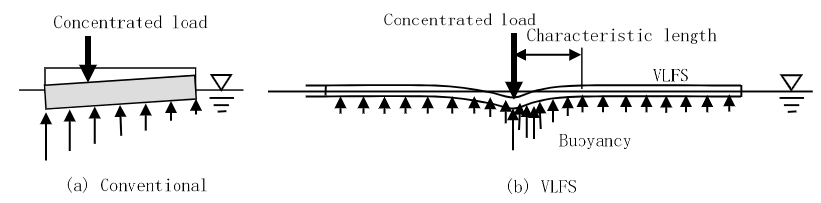
\includegraphics[width=0.7\linewidth]{summer/fluid-tructure-interactions/day2.01.png}
        \caption{弾性支床上の梁モデルの概念図}
        \label{fig:vlfs_concept}
    \end{figure}
    
    前回の授業で“弾性支床上の梁モデル“について検討した。ここで,$EI$ は単位幅あたりの曲げ剛性を,$k_r$ は単位面積当たりの復原力係数を表す。浮体中央に原点を取る。
    \begin{equation}
        EI\frac{d^4W}{dx^4}+k_rW=f \label{eq:beam_on_elastic_foundation}
    \end{equation}
    (1) 式(*)の斉次解が以下で与えられることを確認しなさい(復習,合計4つ)。αの定義については前回の資料を参照。
    \begin{equation}
        W_1 = \exp{\frac{ax}{\sqrt{2}}}\cos{\frac{ax}{\sqrt{2}}}, 
        W_2 = \exp{\frac{ax}{\sqrt{2}}}\sin{\frac{ax}{\sqrt{2}}}, 
        W_3 = \exp{\frac{-ax}{\sqrt{2}}}\cos{\frac{ax}{\sqrt{2}}}, 
        W_4 = \exp{\frac{-ax}{\sqrt{2}}}\sin{\frac{ax}{\sqrt{2}}}
    \end{equation}

    \subsection*{}
    式(\ref{eq:beam_on_elastic_foundation})において、外力項 $f=0$ とした斉次方程式は以下のようになる。
    \begin{equation}
        EI\frac{d^4W}{dx^4}+k_rW=0
    \end{equation}
    この4階線形常微分方程式の特性方程式は、$W=e^{mx}$ と置くことで得られる。
    \begin{equation}
        EIm^4 + k_r = 0
    \end{equation}
    これを $m$ について解くと、
    \begin{equation}
       m^4 = -\frac{k_r}{EI} 
    \end{equation}
    ここで、$\alpha = \sqrt[4]{\frac{k_r}{EI}}$ と定義する。すると、$m^4 = -\alpha^4$ となる。
    $m$ は $-\alpha^4$ の4乗根であるから、
    \begin{equation}
        m = \alpha \sqrt[4]{-1}
    \end{equation}
    $-1$ の4乗根は、$\frac{1+i}{\sqrt{2}}, \frac{-1+i}{\sqrt{2}}, \frac{-1-i}{\sqrt{2}}, \frac{1-i}{\sqrt{2}}$ の4つである。
    したがって、特性根は以下の4つとなる。
    \begin{equation}
        m = \pm \frac{\alpha}{\sqrt{2}} \pm i\frac{\alpha}{\sqrt{2}}
    \end{equation}
    すなわち、
    \begin{equation}
        m_1 = \frac{\alpha}{\sqrt{2}}(1+i), \quad m_2 = \frac{\alpha}{\sqrt{2}}(1-i), \quad m_3 = \frac{\alpha}{\sqrt{2}}(-1+i), \quad m_4 = \frac{\alpha}{\sqrt{2}}(-1-i)
    \end{equation}
    一般解はこれらの線形結合で表される。実数関数の解を得るためにオイラーの公式を適用すると、
    $e^{m_1 x}$ と $e^{m_2 x}$ の線形結合から、
    \begin{equation}
        e^{\frac{\alpha x}{\sqrt{2}}} \left( C_1 \cos\frac{\alpha x}{\sqrt{2}} + C_2 \sin\frac{\alpha x}{\sqrt{2}} \right)
    \end{equation}
    $e^{m_3 x}$ と $e^{m_4 x}$ の線形結合から、
    \begin{equation}
        e^{-\frac{\alpha x}{\sqrt{2}}} \left( C_3 \cos\frac{\alpha x}{\sqrt{2}} + C_4 \sin\frac{\alpha x}{\sqrt{2}} \right)
    \end{equation}
    が得られる。これらはまさしく問題で与えられた4つの独立な解 $W_1, W_2, W_3, W_4$ に対応する。
    
    \vspace{1cm}
    
    中央部に荷重$P$が作用した場合(荷重$f=P\cdotp \delta(x=0)$ , デルタ関数$\delta$は積分すると$1$になる), 一般解は上記の斉次解の線形結合,つまり
    \begin{equation}
        W=a_1W_1+a_2W_2+a_3W_3+a_4W_4
    \end{equation}
    で得られる。
    
    \vspace{1cm}
    
    (2) 事象が左右に対称と考えて,右半分の領域について考えよう。未知の係数$a_1,a_2,a_3,a_4$は適当な条件を付することで与えられる。今回の場合,付するべき条件は次のようになる。下の4つの式の物理的な意味をそれぞれ与えなさい。
    \begin{equation}
        \frac{d^2w}{dx^2}=0,\ \text{at}\ x=\infty
        \label{eq:m1}
    \end{equation}
    \begin{equation}
        \frac{d^3w}{dx^3}=0,\ \text{at}\ x=\infty
        \label{eq:m2}
    \end{equation}
    \begin{equation}
        \frac{dw}{dx}=0\ \text{at}\ x=0
        \label{eq:m3}
    \end{equation}
    \begin{equation}
        \int_0^{\infty}k_rwdx=\frac{P}{2}
        \label{eq:m4}
    \end{equation}
    例) “浮体の右端が自由端であることからモーメントがゼロになる。モーメントは曲率に曲げ剛性を乗じたものであり,式 \eqref{eq:m1}は曲率ゼロ=右端でモーメントがゼロ“

    \subsection*{}
    \begin{itemize}
        \item[\eqref{eq:m1}] \textbf{式}: 
        
        梁の曲げモーメント $M$ は、$M = EI \frac{d^2w}{dx^2}$ で与えられる。この式は、$x=\infty$、すなわち荷重が作用する点から十分に離れた点では、梁の曲げモーメントがゼロになることを示している。これは、局所的な荷重の影響が無限遠には及ばないという物理的な状況を表している。
        \item[\eqref{eq:m2}] \textbf{式}: 
        
        梁のせん断力 $Q$ は、$Q = \frac{dM}{dx} = EI \frac{d^3w}{dx^3}$ で与えられる。この式は、$x=\infty$ において、せん断力がゼロになることを示している。これも(3)と同様に、荷重の影響が無限遠には及ばないことを意味する。
        \item[\eqref{eq:m3}] \textbf{式}: 
        
        $\frac{dw}{dx}$ は梁のたわみ角(傾き)を表す。荷重が $x=0$ の中央に作用し、問題が左右対称であるため、原点 $x=0$ での梁の傾きはゼロになる。この式は、その対称性を表す条件である。
        \item[\eqref{eq:m4}] \textbf{式}: 
        
        $k_r w(x)$ は、位置 $x$ における単位長さあたりの復元力(浮力)を表す。これを右半分($0$ から $\infty$)で積分したものは、梁の右半分に作用する全復元力(全浮力)となる。一方、全荷重 $P$ は左右に均等に支えられるため、右半分が支えるべき荷重は $P/2$ となる。したがって、この式は、梁の右半分における復元力と外力の釣り合いを示している。
    \end{itemize}
    
    \vspace{1cm}
    
    (3) (1)の斉次解のうち,$x=\infty$での境界条件を満たすものは,$W_3,W_4$である。特徴を調べるために$W_3$の形状を描きなさい。エクセルなどのツールを使って構わない。ここでは$\frac{a}{\sqrt{2}}=1$としてよい。
    
    \subsection*{}
    条件より、$W_3(x) = e^{-x} \cos(x)$ のグラフを描画する。この関数は、$x$ が増加するにつれて振幅が $e^{-x}$ に従って指数関数的に減衰する振動(減衰振動)を示す。その形状を以下に示す。
    
    % \usepgfplotslibrary{fpu} ← この行は消すか、行頭に%をつけてコメントアウト!

\begin{figure}[H]
    \centering
    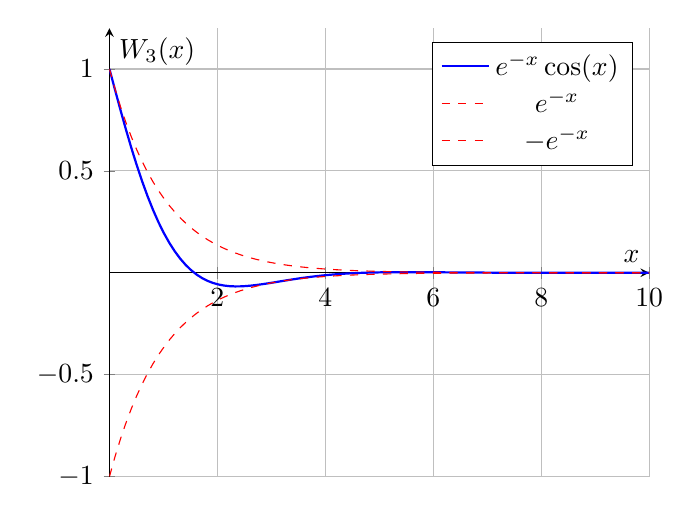
\begin{tikzpicture}
        \begin{axis}[
            axis lines=middle,
            xlabel=$x$,
            ylabel={$W_3(x)$},
            xmin=0, xmax=10,
            ymin=-1, ymax=1.2,
            samples=100,
            legend pos=north east,
            grid=major,
        ]
        \addplot[blue, thick, domain=0:10] {exp(-x)*cos(deg(x))};
        \addplot[red, dashed, domain=0:10] {exp(-x)};
        \addplot[red, dashed, domain=0:10] {-exp(-x)};
        
        % ↓↓↓ 犯人はコイツ!安全な書き方に修正!
        \legend{$e^{-x}\cos(x)$,$e^{-x}$,$-e^{-x}$}
        
        \end{axis}
    \end{tikzpicture}
    
    % ↓↓↓ こっちも念のため修正!
    \caption{関数 $W_3(x) = e^{-x}\cos(x)$ のグラフ}
    
\end{figure}
    
    \vspace{1cm}
    
    ここからは具体的にポンツーン型メガフロートの場合を考えてみる。メガフロートの構造は巨視的には図の〇を付けた二重底部分と類似である。
    
    \begin{figure}[H]
        \centering
        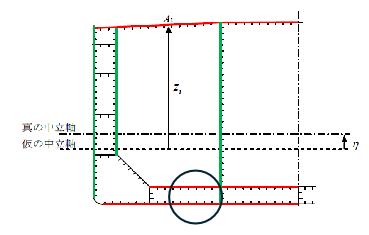
\includegraphics[width=0.7\linewidth]{summer/fluid-tructure-interactions/day2.02.png}
        \caption{二重底構造の模式図}
        \label{fig:double_bottom}
    \end{figure}
    
    (4) 実際の$a$の値がどの程度になるか考えてみる。板厚$t$の二つの板(上側とした側,デッキとボトム)の間の間隔が$H$と考えるとメガフロートの単位幅当たりの断面二次モーメントは,近似的に
    \begin{equation}
        I=\frac{H^2}{2}t \label{eq:moment_of_inertia}
    \end{equation}
    で与えられる。これを説明しなさい。実際には縦隔壁などが存在するので,式(7)は断面二次モーメントの下限の推定値を与える。
    
    \subsection*{}
    断面二次モーメントは、断面の形状に関する量であり、曲げにくさを表す指標である。その定義は $I = \int_A z^2 dA$ で与えられる。ここで $A$ は断面積、$z$ は中立軸からの距離である。
    
    メガフロートの二重底構造を、厚さ $t$、単位幅(幅1)を持つ2枚の板が距離 $H$ だけ離れて配置されているとモデル化する。対称性から、中立軸は2枚の板のちょうど中央、すなわち各板から $H/2$ の距離に位置する。
    
    このモデルにおいて、板自体の厚みは $H$ に比べて十分小さいと仮定し、板自身の断面二次モーメント(図心軸まわりの断面二次モーメント)は無視する。平行軸の定理 $I = I_c + A d^2$ (ここで $I_c$ は図心軸まわりの断面二次モーメント、$A$ は断面積、$d$ は図心と全体の断面の中立軸との距離)を適用する。
    
    \begin{itemize}
        \item 上側デッキプレートの断面二次モーメント $I_{upper}$:
        断面積 $A = t \times 1 = t$、中立軸からの距離 $d = H/2$ であるから、
        $$ I_{upper} \approx A \cdot d^2 = t \left( \frac{H}{2} \right)^2 = \frac{tH^2}{4} $$
        
        \item 下側ボトムプレートの断面二次モーメント $I_{lower}$:
        同様に、断面積 $A=t$、中立軸からの距離 $d = -H/2$ であるから、
        $$ I_{lower} \approx A \cdot d^2 = t \left( -\frac{H}{2} \right)^2 = \frac{tH^2}{4} $$
    \end{itemize}
    
    全体の断面二次モーメント $I$ は、これらの和として与えられる。
    $$ I = I_{upper} + I_{lower} = \frac{tH^2}{4} + \frac{tH^2}{4} = \frac{tH^2}{2} $$
    したがって、式(\ref{eq:moment_of_inertia})が説明される。
    
    \vspace{1cm}
    
    (5) 板厚が$t=20mm(=0.02m)$程度,$H=4m$と考えたときの曲げ剛性 ($=EI,E=\text{スチールの弾性係数}$で $2\times10^{11}\ N/m^2$の値を計算し,さらにポンツーン型浮体の(単位面積当たり)復原力係数は$k_r=9800\  N/m^3$であることから,$\frac{\sqrt{2}}{\alpha}$の値を求めなさい。
    
    \subsection*{}
    与えられた値を用いて、各値を順に計算する。
    
    \begin{enumerate}
        \item \textbf{単位幅当たりの断面二次モーメント $I$ の計算}:
        式(\ref{eq:moment_of_inertia})に $t=0.02 \text{ m}$, $H=4 \text{ m}$ を代入する。
        $$ I = \frac{H^2}{2}t = \frac{(4 \text{ m})^2}{2} (0.02 \text{ m}) = \frac{16}{2} \times 0.02 \text{ m}^3 = 0.16 \text{ m}^4/\text{m} $$
        
        \item \textbf{単位幅当たりの曲げ剛性 $EI$ の計算}:
        スチールのヤング率 $E = 2.0 \times 10^{11} \text{ N/m}^2$ を用いる。
        $$ EI = (2.0 \times 10^{11} \text{ N/m}^2) \times (0.16 \text{ m}^4) = 3.2 \times 10^{10} \text{ Nm}^2 $$
        
        \item \textbf{$\alpha$ の計算}:
        $\alpha$ の定義 $\alpha = \sqrt[4]{\frac{k_r}{EI}}$ に、復原力係数 $k_r = 9800 \text{ N/m}^3$ と上記で計算した $EI$ を代入する。
        $$ \alpha = \sqrt[4]{\frac{9800 \text{ N/m}^3}{3.2 \times 10^{10} \text{ Nm}^2}} = \sqrt[4]{3.0625 \times 10^{-7}} \text{ m}^{-1} \approx 0.02355 \text{ m}^{-1} $$
        
        \item \textbf{$\frac{\sqrt{2}}{\alpha}$ の計算}:
        最後に、求める値を計算する。
        $$ \frac{\sqrt{2}}{\alpha} \approx \frac{1.4142}{0.02355 \text{ m}^{-1}} \approx 60.05 \text{ m} $$
    \end{enumerate}
    
    よって、求める値は $\frac{\sqrt{2}}{\alpha} \approx 60.1 \text{ m}$ となる。
    
    \vspace{1cm}
    
    (6) (3)で描いた図を$x$軸方向に$\frac{\sqrt{2}}{\alpha}$倍すると,メガフロートの変形になる。この点で$\alpha$は縮尺係数のようなものである。このことを念頭において,特性距離$\lambda_s=2\pi\sqrt[4]{\frac{EI}{k_r}}$はどのような物理的意味があるかを述べなさい。
    
    \subsection*{}
    特性距離 $\lambda_s$ の式は、(1)で定義した $\alpha = \sqrt[4]{\frac{k_r}{EI}}$ を用いると、以下のように書き換えられる。
    $$ \lambda_s = 2\pi\sqrt[4]{\frac{EI}{k_r}} = \frac{2\pi}{\alpha} $$
    一方、浮体の変形(たわみ)を表す解は、$e^{-\frac{\alpha x}{\sqrt{2}}}\cos(\frac{\alpha x}{\sqrt{2}})$ のような減衰振動の形をしている。この振動の波長 $L_w$ は、位相項が $2\pi$ 変化する距離に対応するため、$\frac{\alpha L_w}{\sqrt{2}} = 2\pi$ を満たす。これを解くと、$L_w = \frac{2\sqrt{2}\pi}{\alpha}$ となる。
    
    これらから、特性距離 $\lambda_s$ と波長 $L_w$ の間には $L_w = \sqrt{2}\lambda_s$ という関係があることがわかる。
    
    物理的に、特性距離 $\lambda_s$ は、\textbf{局所的な荷重による変形が、構造の曲げ剛性($EI$)と水の復元力($k_r$)のバランスによってどの程度の範囲まで影響を及ぼすかを示す、特徴的な長さ(Characteristic Length)}である。
    具体的には、
    \begin{itemize}
        \item $\lambda_s$ は、荷重によるたわみが減衰しながら振動する波形の「波長」に比例する量であり、変形が空間的に変動する際の基本的なスケールを決定する。
        \item 曲げ剛性 $EI$ が大きいほど、あるいは復元力係数 $k_r$ が小さいほど、$\lambda_s$ は大きくなる。これは、硬くて浮力の影響が相対的に小さい構造ほど、変形がより遠方まで緩やかに伝わることを意味する。
        \item 逆に、柔らかく浮力の影響が大きい構造では $\lambda_s$ は小さくなり、変形は荷重の作用点近傍に局在化する。
    \end{itemize}
    このように、$\lambda_s$ は浮体の構造と流体の相互作用によって決まる、変形現象の空間的なスケールを代表する物理量であると言える。

\vspace{2cm}
今回、\LaTeX の勉強のためにOverLeafを用いて作成しました。
\end{document}